\begin{jointwork}\label{ch:OurWorkflow}
	The main goal of the market simulation framework is to provide a simple-to-use but powerful tool for training RL algorithms on highly configurable markets for users in both a research and a business context. To achieve this, multiple components had to be developed and connected to create the workflow we now provide. This section will introduce the most important parts of the workflow.
\end{jointwork}

When working with our simulation framework, users can choose from two options: First, it is possible to use our tool via a custom Command line interface (CLI). Alternatively, users can interact with the framework through a web-interface, which utilizes Docker for remote-deployment of tasks issued by the user. For detailed insights into our web-interface and remote deployment, see \cite{JudithThesis}.

\Cref{fig:WorkflowSwimlanes} depicts the common workflow activities in our framework. For all possible tasks, the user needs to provide configuration files, which define both the task to be worked on and parameters which influence market and agent behaviour (see \bfref{sec:ConfigureRun}). After the configuration files have been validated, the simulation framework initialized the requested marketplace and agents, and then starts the requested task, for which there are currently three options provided through the CLI or web-interface: \emph{Training}, \emph{Agent-monitoring} and \emph{Exampleprinter}. You may have noticed that one of our monitoring tools is missing from this list, the \emph{Policyanalyser}. As is mentioned in \bfref{subsec:FuturePolicyAnalyser}, this tool must unfortunately still be started manually by the user, as it has not been integrated into the rest of the workflow yet.

At the end of the respective task, the user is always provided with the various diagrams and data (e.g. trained RL models) collected during the respective task, which can then be used in subsequent tasks.

\section{Configuring the run}\label{sec:ConfigureRun}

\begin{figure}[t]
	\centering
	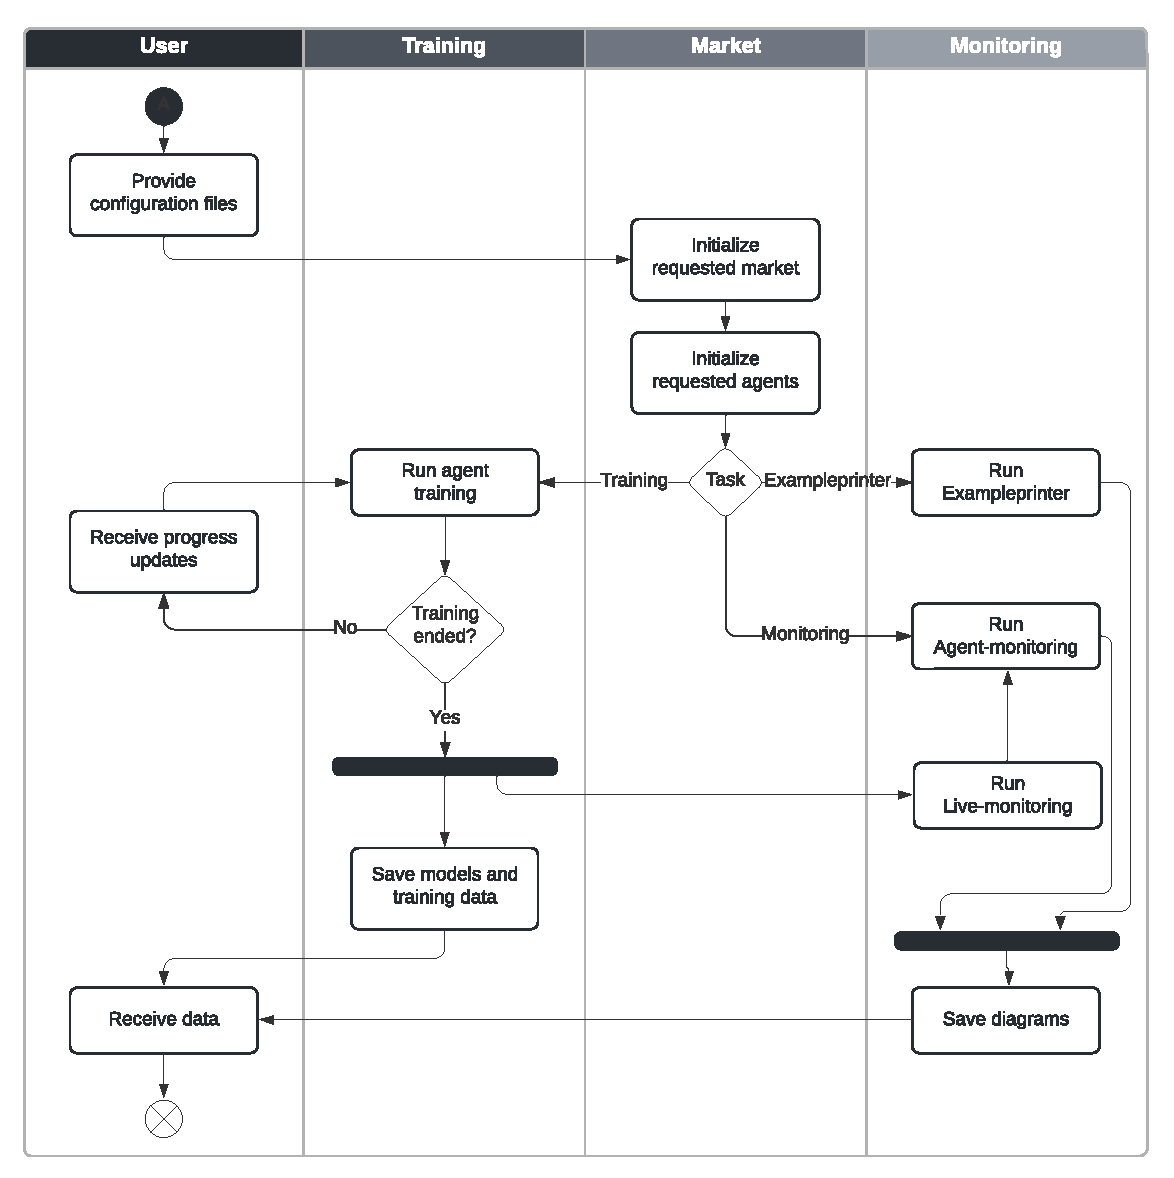
\includegraphics[width = \textwidth]{images/workflow_swimlanes.pdf}\\
	\caption{Diagram depicting possible workflows without webserver interaction.}\label{fig:WorkflowSwimlanes}
\end{figure}

Configuration is one of the most important aspects of the workflow. Without it, each simulation and training session would produce similar, if not the same results. By tweaking different parameters of a run, market dynamics can be changed and agent behaviour and thereby performance be influenced. The goal of our monitoring tools is to enable users to assess the extent to which each parameter influences certain characteristics of the training and/or monitoring session, and to enable them to make informed decisions for subsequent experiments.

Ultimately, all configuration is done using various \texttt{.json} files which contain key-value pairs of the different configurable items. We further differentiate between different groups of configurations, which means that hyperparameters influencing the market, such as maximum possible prices or storage costs, are being handled separate from parameters needed for RL agents, such as their learning rates, allowing users to easily change and tweak parameters involving different parts of the framework. Examples of such configuration files can be found in \bfref{sec:AppendixConfigFiles}.

% Our main goals when building our configuration tools were to make sure that users are able to quickly and safely configure their experiments in a way that is also easily reproducible. To be as user-friendly as possible, a lot of validation logic has been implemented to be able to catch invalid configurations as early as possible, making sure that whenever a training session is started, it is confirmed that the configuration is valid and the training will not fail due to wrongly set parameters at any point. Since our project has also been deployed to a remotely accessible, high-performant machine, we decided on creating an approachable web-interface for our configuration tools, which can now be used for both configuring, starting and evaluating experiments.

% \subsection*{The webserver/Docker-API}\todo{Judith: `Das ganze wie nutze ich die Konfiguration auf dem Webserver könntest Du meiner Meinung nach kürzer fassen'}

% \todo{Example screenshot of the webserver. Configuration and running page?}
% On our webserver, users can upload .json files containing any number of (valid) key-value pairs, or create configurations using a self-validating form, always making sure that it contains only valid values. For example, if the user chooses a Circular Economy market scenario with rebuy prices enabled, the user will not be able to configure agents that cannot operate on such a market.

% Aside from uploading or configuring complete, ready-to-go configurations, users can also choose to upload or create partial configurations, which can then be combined with other configuration objects to create a complete, valid configuration. This allows users to create multiple incomplete configurations containing only select parameters and then test all permutations of these configurations to observe the effect the different parameter combinations have on the experiment. \todo{Mention that this currently needs to be done manually, future work section?}

% An example of one such approach can be found below:
% \todo{Example of a mix and match of parameters}

% After having configured the experiment, the webserver also offers the option of starting multiple runs of the same configuration simultaneously. Most of the times this is recommended, as singular runs are prone to misleading results due to the trained agents training with specific market states, which in some cases may lead to behaviour unique to this starting configuration\todo{Example: Two completely different runs with the same configuration}. By running the same configuration multiple times using different starting circumstances for both the agent that is to be trained as well as its competitors, a configuration's effect on the agent's performance can be disconnected from the pseudo-random market states which influence the vendor's decision making processes.

%% This is regarding Reliability. Maybe I can re-use this in the Interpretation-Chapter, but since I removed it from the title/thesis focus, it is sort of too much for this section
% \todo{Is this perhaps too much interpretation for this section?}\todo{Alex: `Zu deiner Anmerkung: Du hast 2 Optionen um so etwas zu betrachten, entweder Mean + Standardabweichung oder Median + Quantile/Dezile bei sehr stark asymmetrischen Verteilungen. Was für deinen Use Case besser ist kann ich nicht ausm Stehgreif sagen ohne die Daten gesehen zu haben'} A configuration can be interpreted as producing `reliable' agents if any number of simulations all converge on similar agent performances (meaning similar mean rewards). The more singular runs diverge from the mean, \todo{mean or median? What do I use?}the more the agent's performance is dependent on the initial market state, meaning that its performance is less stable, as it will produce unpredictable results on new, unknown market scenarios. A higher number of runs that produce agents which perform on similar levels of performance means that the specific configuration, to be exact the parameters responsible for the RL algorithm, produces `reliable' agents: No matter the state of the market, the agent can always be expected to perform on the same level that was observed during the training process, setting prices that lead to similar profits. Reliability is therefore one of the most important factors in determing an agent's overall quality, as the ultimate goal is always to be able to deploy the agent onto the real market, which will always differ from the simulated environments the agent experienced during training, simply due to the fact that real markets are being influenced by so many more parameters than one could model in our, or for that matter any simulation framework. It should be noted that the chosen RL algorithm drives the reliability of a configuration, as many of the other hyperparameters most often have no impact on this aspect of an experiments results.

%% This section is very long but doesn't really add any useful information
% \section{Choosing what to show the user during training}\todo{Alex: `Die Struktur von 5.2 ist mir noch nicht ganz klar, aber da hört dein Draft ja auch auf, insofern ist das wohl harmlos'}

% During the training process, we of course record all actions the different vendors take, both for the training agent and its competitors, be they RL agents as well, or rule-based agents. Market states and events are also being recorded, to be able to match them to the agent's actions later on. Users of course want to have an indicator of how the training run is going so far, both to inform themselves about the total progress of the training, but also about the quality of the agent they are training. We now have to decide what information is shown to the user, making sure that the user is well informed, whilst also holding back on displaying too much information at once to prevent confusion, as the underlying data and states are ever-evolving, leading to many datapoints being invalidated shortly after their creation. This potential overflow of information is the reason why we decided on displaying minimal information to the user while the training session is still running: Training progress and current performance, in the form of the current overall mean profit.

% The first choice and a save bet when looking at datapoints that will be shown to users is the current training progress. Each training run is defined in its length by a parameter that sets the number of episodes that should be simulated. Each episode consists of an independently initialized market state on which a configurable amount of steps is run. Within each step, the vendors take turns in observing the current market state and then setting their prices for the new and refurbished products and depending on the chosen marketplace, a rebuy price.\todo{Should episodes and steps be defined/explained earlier than this? In the introduction? Specific section/Chapter for important terms and phrases?} We use the training progress to drive the frequency with which data is being shown to the user using the console: Every 10 episodes, we output the current progress, containing both the current number of steps and episodes completed, as well as the mean reward over all episodes the agent has completed. Additionally, to give a more visual component to the training progress a progress bar is displayed, which also tries to estimate the training-time remaining, based on the previous length the simulation of an episode took.

% Using only these two datapoints, the user knows the two most important things: How far along in the training process they are, and how the agent is currently performing.

% \todo{Small paragraph for rl-vs-rl and self-training having different output}

\section{The monitoring workflow}

Within the recommerce workflow, there are two points in time when our monitoring tools are or can be used. While a training session is running, the TensorBoard tool is automatically used to record metrics and give insights into the current training run, by creating visualizations of current market states. By saving intermediate models, the Live-monitoring enables the user to compare agent models saved at different times within the training process, after it has concluded. This can be especially useful when trying to determine the most effective amount of training steps after which a model does not improve further, to optimize future runs. After the training has finished, or at any point disconnected from a training session, our tools described in \bfref{sec:CompleteAgents} can be used to further analyse the trained models. If a training session is terminated by the user before it has completed, the Live-monitoring tool will not be run, but all intermediate models saved up to that point can still be used to monitor the agent's policy at that point in time. The next chapter, \cbfref{ch:AnalysingGraphs}, is dedicated to the monitoring workflow, where we will first run a training session, and then monitor and evaluate the results we get from it.

% \subsection*{After training}

% As has been mentioned before, the end-goal of users using the simulation framework is to be able to deploy trained agents into real markets to set prices independent of human input or guidance. Starting from this premise, the goal of the training process is therefore to model the marketplace as realistically as possible, so that the trained agents can transfer the knowledge from their training to the real market `without noticing a difference'. Before deploying agents to the real market, they need to be tested on their reliability and robustness, to make sure that their policies are not just effective under certain circumstances, but that they are also able to adapt to different market scenarios and behave accordingly.